\documentclass{standalone}

\usepackage{fontspec}
\usepackage[dvipsnames]{xcolor}
\usepackage{tikz}
\usepackage[skins]{tcolorbox}

\definecolor{paper}{HTML}{F1EBDB}
\definecolor{eyered}{HTML}{624442}
\usepackage{eso-pic}

\begin{document}
%\pagecolor{paper}
%\AddToShipoutPictureBG{
%	\begin{tikzpicture}[remember picture, overlay]
%		\draw[fill stretch image=Images/paper_texture_vertical.png]  (current page.south west) rectangle (current page.north east);
%	\end{tikzpicture}
%}
\begin{tikzpicture}
\clip (-6.3cm, -5cm) rectangle (6.3cm, 5cm);
\node[inner sep=0pt] at (0.5cm,-0.65cm) {\includegraphics[scale=0.475]{Images/ink_dragon.png}};

\setmainfont[Scale=3.5]{Dark Crystal-Outline}
\huge
%\node[inner sep=0pt] at (0,3.5cm) {Parliament};%
%\node[inner sep=0pt] at (0,-3.875cm) {of Dragons};
%\node at (3cm,-0.9cm) {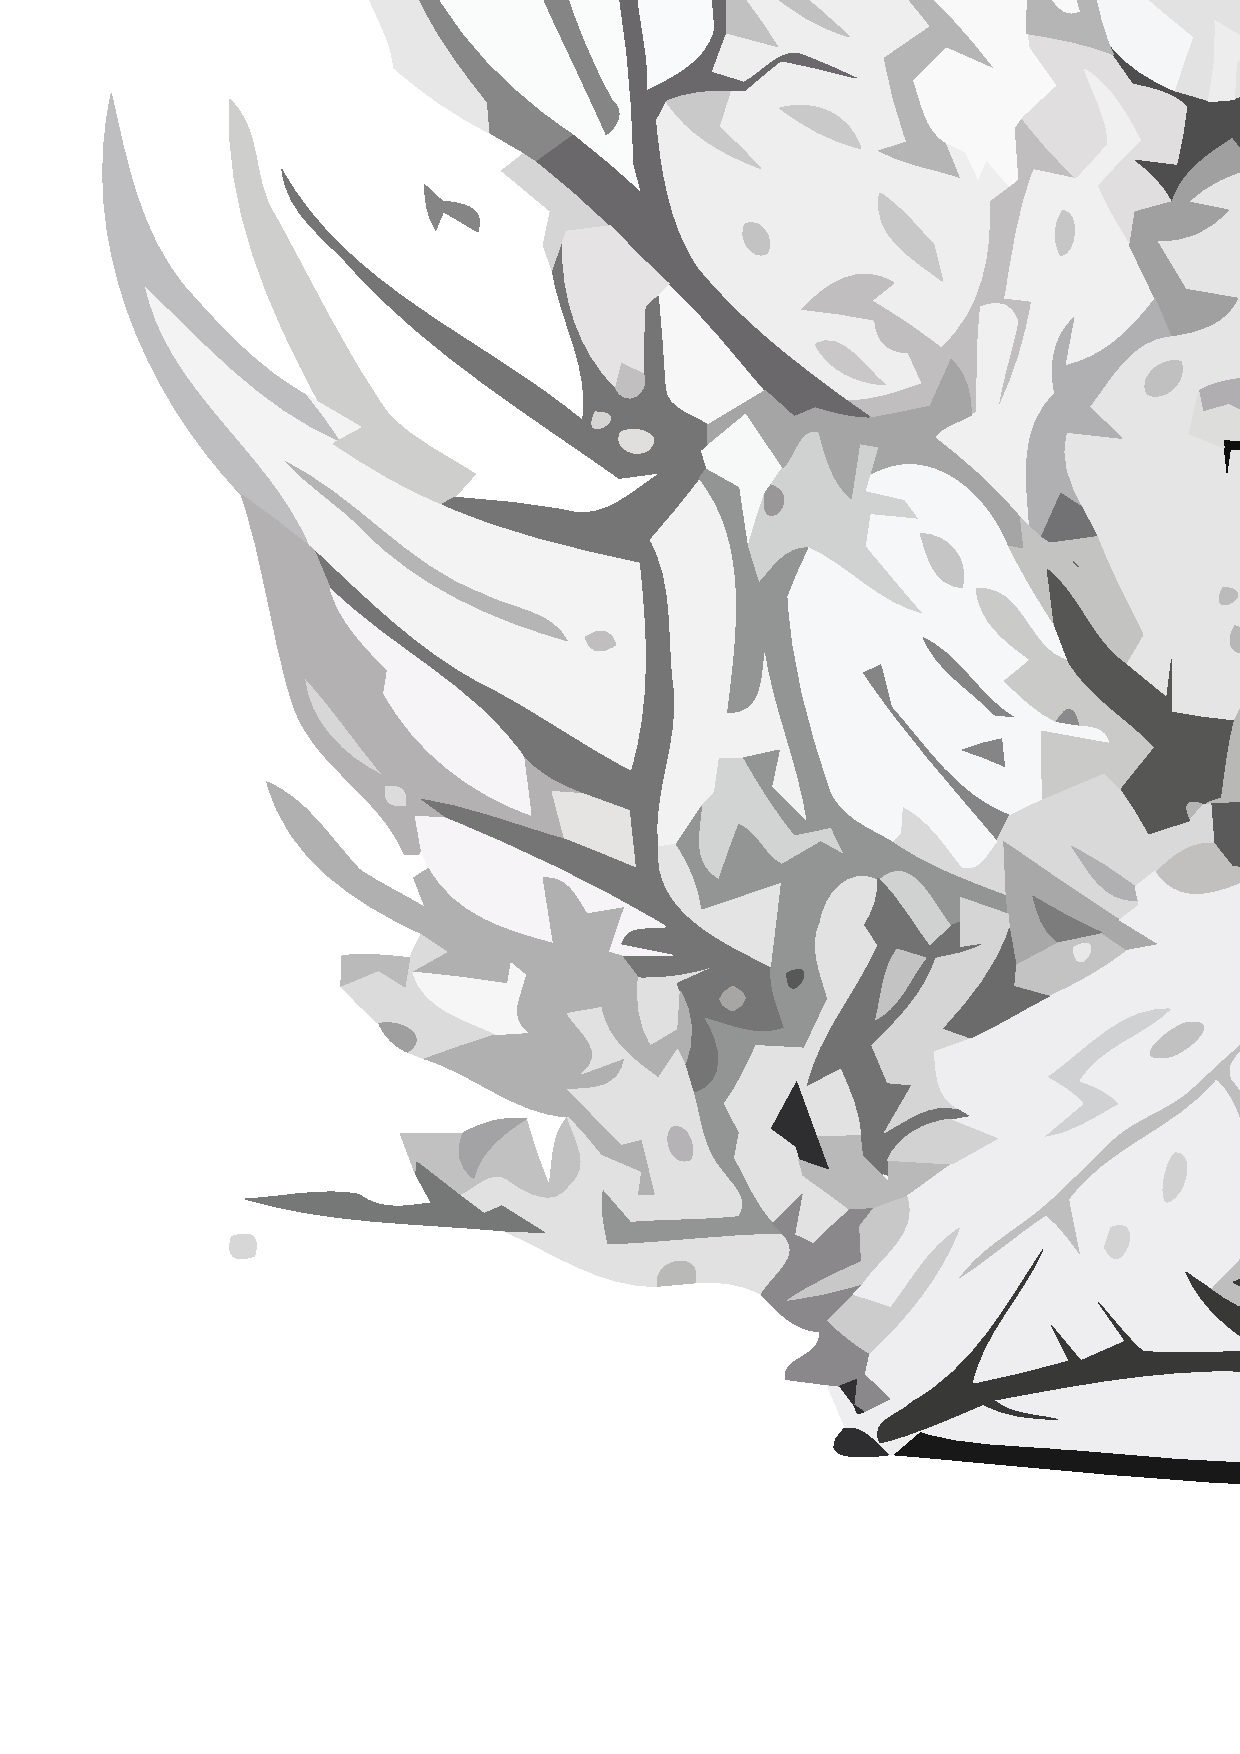
\includegraphics[scale=0.045]{Images/dragon_on_rocks.png}};
\setmainfont{Tex Gyre Chorus}
\LARGE
%\node[inner sep=0pt] at (0,-4.125cm) {A Scoratic Worldbuilding Game by Michael Purcell};
\end{tikzpicture}

\end{document}